\chapter{Aggregated Signature-Based Set Membership Proofs}
\label{ch:AggSM}
\label{sec:ConstructAggregation}
%TODO fix intro
%In the previous chapter, a definition of aggregated set membership proofs was presented and also the requirements it should fulfil. 
This chapter presents a construction of aggregated set membership proofs derived from the non-interactive signature-based set membership proofs, \cite{RANGE-SET}.   In section \ref{sec:SecurityAggregation} it is proved that the aggregation is sound and in section \ref{sec:CSZKAgg} the completeness, soundness and zero-knowledge requirements, stated in the chapter \ref{ch:generalAgg}, is proved to hold for the aggregated signature-based set membership proofs.
%It is seen that the verification algorithm in Construction \ref{alg:VAHSS-HSS-RP} will be time consuming, since each client is verified individually. Therefore a desired property for the above presented server and clients verifiable AHSS would be to aggregate the range proofs into one, since then the verifier would have to perform one range proof verification instead of one for each client as in Construction \ref{alg:VAHSS-HSS-RP}. This would decrease the runtime for the verification significantly, especially in implementations where many clients participate. 
%TODO require the aggregated to filfil def 4. 
%Aggregating the range proofs would require the proofs to be homomorphic, such that the verification remains valid also for an aggregated proof.

%Argument security of aggregation 
\section{Construction}
%The previous section proposed a design of the algorithm \textbf{Aggregate}, such that the  public signature based set memberships proofs could be partly aggregated. 
Construction \ref{alg:ZKSM-Agg} presents an aggregated signature-based set membership proof, derived from the non-interactive signature-based set membership proofs \cite{RANGE-SET}.

The algorithm \textbf{Aggregate}, in Construction \ref{alg:ZKSM-Agg}, partly aggregates a group of set membership proofs by constructing the aggregated proof,
$\Sigma_a $. The aggregated values $D_a,z_{x_a},z_{R_a}$ in $\Sigma_a$ are computed according to Equation \eqref{eq:aggDn}. 

\begin{equation}
\begin{aligned}
\label{eq:aggDn}
D_a &=\prod_{i\in\mathcal{S}}  D_i ^{\prod_{\substack{j\in\mathcal{S}\\ j\neq i}} c_j }  =  g ^ {\sum_{i\in\mathcal{S}} \Big(\prod_{\substack{j\in\mathcal{S}\\ j\neq i}}   c_j \Big)s_i} h^ {\sum_{i\in\mathcal{S}} \Big(\prod_{\substack{j\in\mathcal{S}\\ j\neq i}}   c_j \Big)m_i}
 \\
z_{x_a} &= \sum_{i\in\mathcal{S}} \Big( \prod_{\substack{j\in\mathcal{S}\\ j\neq i}} c_j \Big) z_{x_i} = \sum_{i\in\mathcal{S}} \Big( \prod_{\substack{j\in\mathcal{S}\\ j\neq i}} c_j \Big)s_i - \big( \prod_{j\in\mathcal{S}} c_j \big) \sum_{i\in\mathcal{S}} x_i
\\
z_{R_a} &=  \sum_{i\in\mathcal{S}}  \Big( \prod_{\substack{j\in\mathcal{S}\\ j\neq i}} c_j \Big) z_{R_i} = \sum_{i\in\mathcal{S}} \Big( \prod_{\substack{j\in\mathcal{S}\\ j\neq i}} c_j \Big)m_i - \big( \prod_{j\in\mathcal{S}} c_j \big) \sum_{i\in\mathcal{S}} R_i 
\end{aligned}
\end{equation}

The set $\mathcal{S}$ denotes the index set of the provers and each prover $p_i$ $i\in\mathcal{S}$ publishes a set membership proof $\Sigma_i = (V_i,a_i,D_i,z_{x_i},z_{\tau_i},z_{R_i})$ constructed according to the algorithm \textbf{Prove}. %For all $i\in\mathcal{S}$ the proof $\Sigma_i$ published by the prover $p_i$ is on the form, $\Sigma_i = (V_i,a_i,D_i,z_{x_i},z_{\tau_i},z_{R_i})$.
The challenges, denoted $c_i$ for $i\in\mathcal{S}$, are computed according to the algorithm \textbf{CalculateChallenges}.

The above aggregation has the computational complexity $\mathcal{O}(|\mathcal{S}|^2)$. This is reduced to be linear in $|S|$, by considering the following optimization. Instead of computing the product $\prod_{\substack{j\in\mathcal{S},\: j\neq i}} c_j $ for each $i$, it is sufficient to compute the product $c=\prod_{\substack{j\in\mathcal{S}}} c_j $  once and then the truncated product can be obtained by noting that $ \prod_{\substack{j\in\mathcal{S},j\neq i}} c_j = c/c_i $. Thereby, for each $i\in\mathcal{S}$, it is sufficient to perform one division instead of computing the product $\prod_{\substack{j\in\mathcal{S},\:j\neq i}} c_j $.

Due to the aggregation, the equality $D_a=C^ch^{z_{R_a}}g^{z_{x_a}}$ is checked once instead of once for each proving party in the protocol. This can bee seen by comparing the algorithm \textbf{Verify} in Construction \ref{alg:ZKSM-Agg} with running the algorithm \textbf{Verify} in Construction \ref{alg:ZKSM} once for each prover. 

\begin{algorithm}[]
\caption{\textbf{: Aggregation of non interactive set membership proof}}
\textbf{Goal:}  Given the Pedersen commitments $C_i=g^{x_i} h^{R_i}$, for $i\in\mathcal{S}$. The construction  proves that all secrets $x_i$ belong to the set $\Phi$, without revealing anything else about the secrets.
\vspace{2pt} 
\hline 
\vspace{2pt}
\begin{itemize}
  \item\text{\textbf{SetUp} $(1^\lambda,\Phi)\xrightarrow[]{}(sk,pp)$}\\
 Let g be a generator of the group $\mathds{G}$ and $h$ an element in the group such that $log_g(h)$ is unknown.  
Pick uniformly at random $\chi\in_R\mathds{F}$ and put $sk=\chi$. Define $y=g^\chi$ and $A_i=g^{\frac{1}{\chi+i}} \:\forall i\in\Phi$, output $pp=(g,h,y,\{A_i\}_{i\in\Phi})$.

\item\text{\textbf{Prove} $(pp,i,C_i,x_i,\Phi)\xrightarrow[]{}\Sigma_i$}\\
Pick uniformly at random $\tau_i\in_R\mathds{F}$, choose from the set $\{A_i\}$ the element $A_{x_i}$ and calculate $V_i=A_{x_i}^{\tau_i}$. Pick uniformly at random three values $s_i,t_i,m_i\in_R\mathds{F}$. Put $a_i=e(V_i,g)^{-s_i}e(g,g)^{t_i}$,  $D=g^{s_i}h^{m_i}$, $c=\text{Hash}(C_i,V_i,a_i,D_i)$ and compute $z_{x_i} = s_i-x_i c_i$, $z_{R_i} = m_i-R_ic_i$ and $z_{\tau_i}= t_i-\tau_i c_i$.  Finally construct and publish the proof $\Sigma_i = (V_i,a_i,D_i,z_{x_i},z_{\tau_i},z_{R_i})$.

\item \text{\textbf{Aggregate} $( pp,\{ \Sigma_i\}_{i\in\mathcal{S}} ) \xrightarrow[]{} \Sigma_a$} \\
Given a set of proofs  $\{\Sigma_i\}_{i\in\mathcal{S}}$. Aggregate the values $( \{D_i \}_{i\in\mathcal{S} }, \{ z_{x_i}\}_{i\in\mathcal{S} }, \{ z_{r_i}\}_{i\in\mathcal{S}  }) \mapsto$ $ D_a,z_{x_a},z_{R_a}$ according to equation \eqref{eq:aggDn}. Construct and publish the aggregated proof $\Sigma_a = (\{V_i\}_{i\in\mathcal{S} },\{a_i\}_{i\in\mathcal{S} },D_a,\{z_{x_i}\}_{i\in\mathcal{S} }, z_{x_a}, \{z_{\tau_i}\}_{i\in\mathcal{S} },z_{R_a})$.

\item \text{ \textbf{CalculateChallenges} $(\{C_i\}_{i\in\mathcal{S}},\{\Sigma_i\}_{i\in\mathcal{S}} ) \xrightarrow[]{} \{c_i\}_{i\in\mathcal{S}}$ }\\
For all $i\in\mathcal{S}$ parse the proof $\Sigma_i$, then compute the challenge $c_i = Hash(C_i,V_i,a_i,D_i)$. Finally output the set of all challenges $\{c_i\}_{i\in\mathcal{S}}$. 

\item\text{\textbf{Verify} $(pp,\Sigma_a,\{C_i\}_{i\in\mathcal{S}},\{c_i\}_{i\in\mathcal{S}}) \xrightarrow[]{} \{0,1\}$} \\
Compute the product of the challenges $c=\prod_{i\in\mathcal{S}} c_i$. Check if $D_a\overset{?}{=} \big( \prod_{i\in\mathcal{S}}C_i\big)^ch^{z_R_a}g^{z_x_a}\wedge a_i \overset{?}{=} e(V_i,y)^c_i e(V_i,g)^{-z_{x_i}}e(g,g)^{z_{\tau_i}}$ for all $i\in\mathcal{S}$. If the equalities hold return $1$ otherwise return $0$.
\end{itemize}
\label{alg:ZKSM-Agg}
\end{algorithm} 


In Construction \ref{alg:ZKSM-Agg} the algorithm \textbf{Prove} is run by all provers, the algorithm \textbf{Aggregate} is run by the aggregating party and the algorithm \textbf{Verify} is performed by the verifier. The algorithm \textbf{SetUp} is assumed to be performed in advance by a trusted party.

In the aggregated signature-based set membership proof the challenges are given as input to the verification algorithm, unlike Construction \ref{alg:ZKSM} where they are computed in the verification algorithm. This raises the question, which party should be responsible for computing the challenges?  It is not desired that the party performing the aggregation computes the challenges, since it creates opportunities for cheating. For the same reason the proving parties  should not compute the challenges. Thereby, the algorithm \textbf{CalculateChallenges} in Construction \ref{alg:ZKSM-Agg} is assumed to be performed by an honest party independent of both the proving parties and the aggregating party. 

Another alternative is to provide the entire proofs $\{\Sigma_i\}_{i\in\mathcal{S}}$ as input to the verification algorithm, enabling the verifier to compute the challenges. This would consequently increase the computations required by the verifier. For the rest of this paper, if nothing else is mentioned, it is assumed that the algorithm \textbf{CalculateChallenges} is performed according to Construction \ref{alg:ZKSM-Agg} by a trusted party. 

%Comparing the algorithm \textbf{VerifyAggregatedProof} with performing the algorithm \textbf{Verify} in set membership construction once for each clients, it is seen that the first equality check $D \overset{?}{=}( \prod_{i=1}^n C_i )^{c}h^{z_R}g^{z_x}$ is done once instead of once for $|\mathcal{S}|$ times. Construction \ref{alg:ZKSM-Agg} presents all algorithms ,  \textbf{Prove}, \textbf{Aggregate}, \textbf{CalulateChallenges} and \textbf{VerifyAggregatedProof}, needed to build the aggregated set membership proof. 



% , that verifier all individual set membership proof by performing only one verification, resulted in a that a method for aggregating parts of the set membership proof. This method is compiled in Construction \ref{alg:ZKSM-Agg}, where the set membership proof originally presented in \cite{Efficient_proof_interval} is modified to reduce the computational complexity in applications where multiple  proofs are verified simultaneously.

%This leads to that a verification algorithm for verifying the aggregated version of set membership proofs $RP_i$ for $i\in\mathcal{S}$ to be as the algorithm \textbf{VerifyAggregatedProof} in Construction \ref{alg:ZKSM-Agg}.  %TODO 
%\begin{itemize}
%\item\text{\textbf{VerifyAggregatedProof} $(g,h,\{C_i\}_{i\in\mathcal{S}},\{c_i\}_{i\in\mathcal{S}} ,\texit{proof}_{SM,a}) \xrightarrow[]{} \{0,1\}$} \\
%Compute the product of the challenges $c=\prod_{i\in\mathcal{S}} c_i$. Check if $D_a\overset{?}{=} \big( \prod_{i\in\mathcal{S}}C_i\big)^ch^{z_R_a}g^{z_x_a}\wedge a_i \overset{?}{=} e(V_i,y)^c_i e(V_i,g)^{-z_{x_i}}e(g,g)^{z_{\tau_i}}$ for all $i\in\mathcal{S}$. If the equalities holds the provers has convinced the verifier that $x_i\in\Phi$ for all $x_i$ such that $i\in\mathcal{S}$ return $1$ otherwise return $0$.
%\end{itemize}
 
 
\subsection*{Multiple aggregating parties}
To reduce the computational load of the aggregating party it is possible to split the aggregation between multiple parties. %The computational complexity for the algorithm \textbf{Aggregate} is linear in the number of proofs that are aggregated. 

Let the set $\mathcal{K}$ represent the set of parties performing the aggregation, and the set $\mathcal{S}_k$ represent the assigned set of set membership proofs to the $k^{th}$ aggregating party. The sets $\mathcal{S}_k$ for $k\in\mathcal{K}$ are such that $\bigcup_{k\in\mathcal{K}}\mathcal{S}_k = \mathcal{S}$ and $\mathcal{S}_i\bigcap \mathcal{S}_j= \emptyset$ for all $i,j\in\mathcal{K}$ such that $i\neq j$. 

An aggregated signature-based set membership proof, where the aggregation is split between several parties, is presented in appendix \ref{app:manyAggregatingParties} in Construction \ref{alg:ZKSM-Agg-Many}. The adjustments made compared to Construction \ref{alg:ZKSM-Agg} are: the algorithm \textbf{Aggregate} is performed by each party in the set $\mathcal{K}$ on the input $(pp,\{\Sigma_i\}_{i\in\mathcal{S}_k})$, outputting the aggregated proof $\Sigma_{a_k}$. The algorithm \textbf{Verify} is performed once on the input $(pp,\{\Sigma_{a_k}\}_{k\in\mathcal{K}},\{C_i\}_{i\in\mathcal{S}},\{c_i\}_{i\in\mathcal{S}} )$ and  is modified, compared to Construction \ref{alg:ZKSM-Agg}, such that it verifies multiple aggregated proofs. By letting the set of aggregating parties $\mathcal{K}$ consist of one element $k$, and $\mathcal{S}_k  = \mathcal{S}$ constructions \ref{alg:ZKSM-Agg} and \ref{alg:ZKSM-Agg-Many} are equivalent. 
%TODO elaborate


An illustrative figure of how the aggregation is split between the aggregating parties is seen in Figure \ref{fig:workflow}. Each prover generates a set membership proof, and then sends it to its assigned aggregating party. Then each aggregating party aggregates the received set membership proofs, according to the algorithm \textbf{Aggregate} in Construction \ref{alg:ZKSM-Agg-Many}, and sends the aggregated proof to the verifier. Finally the verifier validates all aggregated proofs.

In Figure \ref{fig:workflow} the computation of the challenges is done by an independent party, which introduces a new party to the scheme. To compute the challenges without introducing a new party the aggregating parties can compute the challenges.  However, as discussed previously the same party that aggregates a set of proofs should not compute the challenges for these proofs. To use the aggregating parties for the computations, assume that they are not collaborating and linked in a closed chain. Then each aggregating party computes the challenges for the set of proofs aggregated by the consecutive party in the chain.  
%As discussed previously it would be possible to have the verifier computing the challenges, by additionally giving the proofs $\{ \Sigma_i\}_{i\in\mathcal{N}}$ as input to the verification algorithm. 


 \begin{figure}
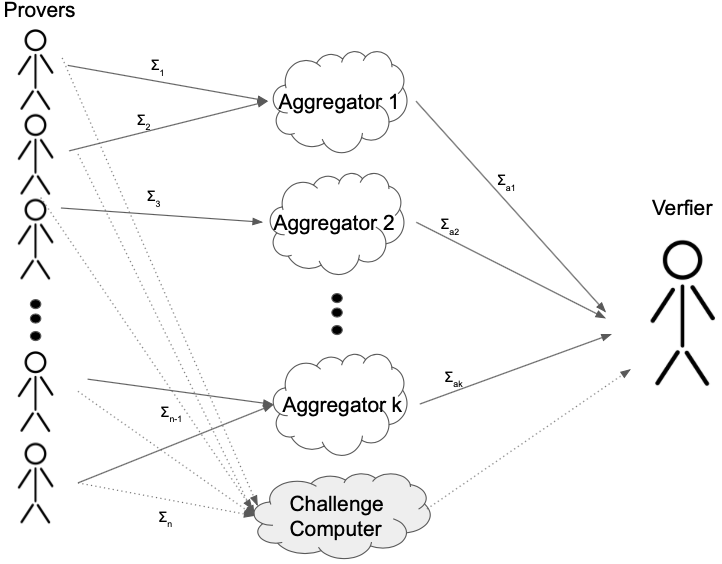
\includegraphics[width=\linewidth]{./figure/splitagg.png}
\caption{Provers outsourcing their set membership proofs to their assigned aggregator that in turn publishes an aggregated set membership proof. }
\label{fig:workflow}
\end{figure} 



%\section{Aggregation of signature based set membership proof}

%In this section the possibility to aggregate the set membership and signature based range proofs  is examined.  The construction of these two are similar and it is sufficient to consider one of them and the conclusion will hold for both constructions. Due to its simpler notation the set membership proof is considered.

%2D example, removed.
\begin{comment}
Again consider the two set membership proofs $\Sigma_1,\Sigma_2$ as defined above, but now restrict the aggregation to only concern half the set membership proof. Namely only terms participating in the the first equality check, $D\overset{?}{=} C^ch^{z_R}g^{z_x}$, in the verification. 

Note that if only a part of the proofs are aggregated it still leads to reduction of computational complexity for the verifier. The goal is now design the aggregation such that the aggregated proof satisfies $D = C^ch^{z_R}g^{z_x}$. 
%Before aggregation calculate the challenges $c_1,c_1$ as $c_i =Hash(D_i,a_i),\:i=1,2$. 
Define the aggregated proof as, $\Sigma_a=(D,z_x,z_R)$, this means the proof does not contain the bilinear maps output $a$ and the group element $V, z_{\tau}$. Further let the the aggregated proof be computed according to, 
\begin{equation}
\label{eq:aggD2}
\begin{aligned}
D &= D_1^{c_2}\cdot D_2^{c_1} = (g^{s_1}h^{m_1}) ^{c_2} \cdot (g^{s_2}h^{m_2}) ^{c_1}  =g^{s_1c_2+s_2c_1}h^{m_1c_2+m_2c_1} \\
z_x &= c_2z_{x_1} +c_1 z_{x_2} = c_2(s_1-x_1c_1)  + c_1(s_2-x_2c_2) = s_1c_2 + s_2c_1 -c_1c_2(x_1+x_2)\\
z_R &= c_2z_{R_1} +c_1 z_{R_2} = c_2(m_1-R_1c_1)  + c_1(m_2-R_2c_2) = m_1c_2 + m_2c_1 -c_1c_2(R_1+R_2)
\end{aligned}
\end{equation}
This construction of the aggregation will result in that the challenges always appears in a product which resolves the problem of them being different. Additionally also define the product of the challenges and commitments as,
\begin{align*}
c &= c_1c_2 \\
C &= C_1C_2 = (g^{x_1}h^{R_1}) (g^{x_2}h^{R_2}) = g^{x_1+x_2}h^{R_1+R_2}.
\end{align*}

%It is assumed that the random values $R_i$ is chosen such that $R_n = \phi(N)\lceil \frac{\sum_{i=1}^{n-1}R_i}{\phi(N)}\rceil- \sum_{i=1}^{n-1}R_i $, which holds for the randomness in a VHASS construction, hence for $i=1,2$ if follows that $R_2 = \phi(N)\lceil \frac{R_1}{\phi(N)}\rceil- R_1$, and thus $h^{c_1c_2(R_1+R_2)} = 1$. 
%This property will not be required for the below calculations, however is does reduce notation and therefore the computations are done under this assumption. 

The aggregated proof $\Sigma_a$, computed according to equation \eqref{eq:aggD2} satisfies the equality $D= C^ch^{z_R}g^{z_x}$, this is seen below,
\begin{align*}
LHS &= D = D_1^{c_2}\cdot D_2^{c_1} =g^{s_1c_2+s_2c_1}h^{m_1c_2+m_2c_1} \\
RHS &= C^ch^{z_R}g^{z_x} = (C_1C_2)^{c_1c_2}h^{c_2z_{R_1}+c_1z_{R_2}}g^{c_2z_{x_1}+c_1z_{x_2}}\\ 
&=(g^{x_1 + x_2})^{c_1c_2} h^{m_1c_2 +m_2c_1} g^{s_1c_2+ s_2c_1- c_1c_2(x_1+x_2)}  \\
&= g^{(x_1+x_2)c_1c_2 - c_1c_2(x_1+x_2) +s_1c_2+s_2c_1} h^{m_1c_2 +m_2c_1} = g^{s_1c_2+s_2c_1} h^{m_1c_2 +m_2c_1} \\
\\ \implies \text{LHS} =\text{RHS}&.
\end{align*}

%This means that this aggregation to construct the proof $RP$ , from the two range proofs $RP_1,RP_2$ as above satisfies the first equality of the verification. 
Aggregation of the two set membership proof defined according to equation  \eqref{eq:aggD2} results in an aggregation that satisfies the  completeness. The next step is to check if this aggregation can be extended to aggregate an arbitrary number of set membership proofs and still satisfy the completeness. 
\end{comment}

%A hint can also be seen in Construction \ref{alg:ZKRP} where the verification of first equity is aggregated while the second is done for each $j\in\mathds{Z}_l$. 




\section{Soundness of Aggregation}
\label{sec:SecurityAggregation}
In this section it is proved that the aggregation must be performed according to the algorithm \textbf{Aggregate} if the aggregated proof $\Sigma_a$ validates true in Construction \ref{alg:ZKSM-Agg}. This is proved under the assumption that: proving parties are not communicating or collaborating between themselves, proving parties are not communicating or collaborating with the aggregating party (or parties), the set membership proof in Construction \ref{alg:ZKSM} is sound and $D_a\neq C^c$.  In this section the product of the Pedersen commitments, $\prod_{i\in\mathcal{S}}C_i$, is denoted $C$ and the product of the challenges, $\prod_{i\in\mathcal{S}} c_i$, is denoted $c$.
%,  where  $C_i$ is a Pedersen commitment of the secret $x_i$ and $c_i$ the challenges used to construct the proofs, $\Sigma_i$, proving that the secret $x_i\in\Phi$, for $i\in\mathcal{S}$. 


If $D_a =  C^c$, it would be possible for an aggregating party to choose the values $D_a,z_{x_a},z_{R_a}$ according to: $D_a =C^c, z_{x_a} = \phi(p), z_{R_a} = \phi(p)$.
%Note that $p$ is the prime underlying the field $\mathds{F}$, $C=\prod_{i\in\mathcal{S}}C_i$ and $c=\prod_{i\in\mathcal{S}}c_i$. 
For the above choice of $D_a,z_{x_a},z_{R_a}$ the equation, $D_a\overset{?}{=} C^c h^{z_{R_a}}g^{z_{x_a}}$ holds trivially true, independent of whether the commitment $C_i$ and the values $z_{x_i}$, thereby $z_{x_a}$, hides the same secret for all $i\in\mathcal{S}$. Therefore it is required that $D_a \neq C^c$.


Under the assumption discussed above, Theorem \ref{thm:aggrgeation} states that the  aggregation must be performed according to the algorithm \textbf{Aggregate} for the algorithm \textbf{Verify} to validate true, in Construction \ref{alg:ZKSM-Agg}. 
\vspace{0.5cm}
\begin{thm}[\textbf{Soundness of aggregation}]
\label{thm:aggrgeation}
Let $\mathcal{A}$ be a PPT adversary. Assume $\mathcal{A}$ has access to the input to the algorithm \textbf{Aggregate} in Construction \ref{alg:ZKSM-Agg} and the Pedersen commitment, $\{C_i\}_{i\in\mathcal{S}}$, but no other information. Assume that the adversary  $\mathcal{A}$ cannot collaborate with the provers, that the provers cannot collaborate with each other and that the set membership proof in Construction \ref{alg:ZKSM} is sound. 

%The provers are not assumed to be honest, but it is assumed that their published proofs are one the form $\Sigma_i = (V_i,a_i,D_i,z_{x_i},z_{\tau_i},z_{R_i})$, where $V_i,D_i\in\mathds{G}$, $a_i\in\mathds{G}_T$ and $z_{x_i},z_{\tau_i},z_{R_i} \in\mathds{F}$, and that the Pedersen commitments $C_i=g^{x_i}h^{R_i}$.


Under these assumptions the adversary $\mathcal{A}$ has a negligible probability of construction $\Sigma_a$ such that: Prob$($\textbf{Verify}$(pp,\Sigma_a,\{C_i\}_{i\in\mathcal{S}},\{c_i\}_{i\in\mathcal{S}}) )=1$, where $D_a\neq C^c$ and  $z_{x_a} \neq \sum_{i\in\mathcal{S}} \Big( \prod_{j\in\mathcal{S}, j\neq i} c_j \big) z_{x_i}$. 


\end{thm}

\begin{proof}
The soundness of signature-based set membership proofs and that the algorithm \textbf{Verify} checks that $a_i\overset{?}{=} e(V_i,y)^{c_i}e(V_i,g)^{-z_{x_i}}e(g,g)^{z_{\tau_i}}$,  for all $i\in\mathcal{S}$, implies that the values $V_i,a_i,z_{x_i},z_{\tau_i}$ of $\Sigma_i$ must be computed according to the algorithm \textbf{Prove} in Construction \ref{alg:ZKSM-Agg}. The values $z_{R_i}$ and $D_i$ are not used directly in the verification, thus the only requirements are that $z_{R_i}\in\mathds{F}$ and $D_i\in\mathds{G}$, for all $i\in\mathcal{S}$.  Assume, without loss of generality that  $D_a=g^\alpha h^\beta$, where $\alpha,\beta\in\mathds{F}$. 

Assume that the adversary $\mathcal{A}$, can construct a valid proof $\Sigma_a$, such that: $D_a\in\mathds{G}$, $z_{x_a},z_{R_a}\in\mathds{F}$ and  $z_{x_a} \neq \sum_{i\in\mathcal{S}} \Big( \prod_{j\in\mathcal{S}, j\neq i} c_j \big) z_{x_i}$. 

%The adversary $\mathcal{A}$ should construct a valid aggregated proof, $\Sigma_a$, i.e choosing the values $D,_az_{x_a},z_{R_a}$. These should be such that $D_a\in\mathds{G}$, $z_x,z_R\in\mathds{F}$ and  $z_{x_a} \neq \sum_{i\in\mathcal{S}} \Big( \prod_{j\in\mathcal{S}, j\neq i} c_j \big) z_{x_i}$. Assume, without loss of generality that  $D_a=g^\alpha h^\beta$, where $\alpha,\beta\in\mathds{F}$. 

For the aggregated proof to be valid it must hold that $D_a= C^ch^{z_{R_a}}g^{z_{x_a}}$ which implies that the values $\alpha,\beta,z_x,z_R$ must satisfy:
\begin{align*}
g^\alpha h^\beta  = C^cg^{z_{x_a}}h^{z_{R_a}}.
\end{align*}
The values of $C^c $ cannot be modified by the adversary since it is sent directly from the provers to the verifier. The Pedersen commitments are assumed to be on the form $C_i= g^{x_i}h^{R_i}$ for all $i\in\mathcal{S}$ and the challenges are correctly computed and checked by a trusted party.

Consequently, by expanding the right hand side of the equality it follows that,
\begin{align*}
g^\alpha h^\beta =  g^{c \sum_{i\in\mathcal{S}}x_i +z_{x_a} } h^{ c \sum_{i\in\mathcal{S}}R_i +z_{R_a}   }.
\end{align*}

If $\alpha \neq c \sum_{i\in\mathcal{S}} x_i+z_{x_a}$ and $\beta\neq c\sum_{i\in\mathcal{S}}R_i +z_{R_a}$, the above equality contradicts to the binding property of the Pedersen commitments.  %assumption that it is not possible to construct two equal Pedersen Commitments hiding different secrets.
Thereby, the values $\alpha,\beta,z_{x_a}$ and $z_{R_a}$ must satisfy: $\alpha =  c\sum_{i\in\mathcal{S}}x_i+z_\x_a}$ and $\beta =  c\sum_{i\in\mathcal{S}}R_i +z_{R_a}$.  

This can be rewritten as $\alpha-z_{x_a} =  c \sum_{i\in\mathcal{S}} x_i$ mod $\Phi(p)$ and  $\beta-z_{R_a} =  c \sum_{i\in\mathcal{S}} R_i$ mod $\Phi(p)$. The sums $ \sum_{i\in\mathcal{S}} x_i$ and $ \sum_{i\in\mathcal{S}} R_i$ are assumed to be unknown.  

Thereby, under the assumption that $z_{x_a}\neq \sum_{i\in\mathcal{S}} \Big( \prod_{j\in\mathcal{S}, j\neq i} c_j \big) z_{x_i} $ the adversary has a negligible probability of choosing $\alpha,\beta,z_{x_a},z_{R_a}$ such that $D_a= C^ch^{z_{R_a}}g^{z_{x_a}}$. It follows that  $z_{x_a} = \sum_{i\in\mathcal{S}} \Big( \prod_{j\in\mathcal{S}, j\neq i} c_j \big) z_{x_i}$, which contradicts the assumption and proves the theorem. 


\end{proof}
Note that the theorem would still hold even if several untrusted parties aggregated subsets of the proofs and a verifier validated all the aggregated proofs. 

\section{Completeness, Soundness and Zero-Knowledge}
\label{sec:CSZKAgg}
In this section, it is proved that Construction \ref{alg:ZKSM-Agg}  fulfils the completeness, soundness and zero-knowledge requirements stated in chapter \ref{ch:generalAgg}. This is proved under the  assumption that the aggregation is performed according to the algorithm \textbf{Aggregate},  provers cannot communicate or collaborate with each other and that Construction \ref{alg:ZKSM} satisfies the requirement stated in Definition \ref{def:ZKP}.
% The assumption that the aggregation is performed by a trusted party %TODO
 The requirements also hold for Construction \ref{alg:ZKSM-Agg-Many}, considering $|\mathcal{K}|>1$.

\subsubsection*{Completeness}
To prove the completeness of Construction \ref{alg:ZKSM-Agg}, it has to be proved that\\ \textbf{Verify}$ ( $\textbf{Aggregate}$ (\{ $\textbf{Prove}$ (pp,i,C_i,x_i,\Phi)\}_{i\in\mathcal{S}}) )= 1$. To prove this, let $\Sigma_i$ for $i\in\mathcal{S}$ denote proofs constructed by the algorithm \textbf{Prove} and $\Sigma_a $ denote the aggregation of these proofs obtained according to algorithm \textbf{Aggregate}. For all $i\in\mathcal{S}$, let $C_i$ denote the Pedersen commitment of the secrets $x_i$ and $c_i$ denote the challenge used in the proof.

Then by the completeness property of the signature-based set membership proof \cite{RANGE-SET}, it holds that:
\begin{align*}
a_i = e(V_i,y)^{c_i}e(V,g)^{z_{x_i}}e(g,g)^{z_{\tau_i}} \:\: \forall \: i\in\mathcal{S}.
\end{align*}

It remains to argue that $D_a =C^ch^{z_{R_a}}g^{z_{x_a}}$, where $C=\prod_{i\in\mathcal{S}}C_i$ and $c=\prod_{i\in\mathcal{S}}c_i$. By construction it holds that:
\begin{align*}
D_a = &g ^ {\sum_{i\in\mathcal{S}} \Big(\prod_{\substack{j\in\mathcal{S}\\ j\neq i}}   c_j \Big)s_i} h^ {\sum_{i\in\mathcal{S}} \Big(\prod_{\substack{j\in\mathcal{S}\\ j\neq i}}    c_j \Big)m_i}  ,
\\
 C^ch^{z_{R_a}}g^{z_{x_a}} =&\:  \Big( \prod_{i\in\mathcal{S}} C_i \Big)^{\prod_{i\in\mathcal{S}} c_i}h^ {\sum_{i\in\mathcal{S}} \Big( \prod_{\substack{j\in\mathcal{S}\\ j\neq i}}   c_j \Big)m_i}
g^{ \sum_{i\in\mathcal{S}} \Big( \prod_{\substack{j\in\mathcal{S}\\ j\neq i}}   c_j \Big)s_i - \big( \prod_{j\in\mathcal{S}} c_j \big) \sum_{i\in\mathcal{S}} x_i}
\\ 
 = &\Big( g^{\sum_{i\in\mathcal{S}} x_i} h^{\sum_{i\in\mathcal{S}} R_i}\Big)^{\prod_{i\in\mathcal{S}} c_i} h^{ \sum_{i\in\mathcal{S}} \Big( \prod_{\substack{j\in\mathcal{S}\\ j\neq i}} c_j \Big)m_i - \big( \prod_{j\in\mathcal{S}} c_j \Big) \sum_{i\in\mathcal{S}} R_i  }
 \\
 &g^{ \sum_{i\in\mathcal{S}} \Big( \prod_{\substack{j\in\mathcal{S}\\ j\neq i}}   c_j \Big)s_i - \big( \prod_{j\in\mathcal{S}} c_j \big) \sum_{i\in\mathcal{S}} x_i} \\
 =  &g^{ \sum_{i\in\mathcal{S}} \Big( \prod_{\substack{j\in\mathcal{S}\\ j\neq i}}  c_j \Big)s_i } h^{\sum_{i\in\mathcal{S}} \Big( \prod_{\substack{j\in\mathcal{S}\\ j\neq i}}   c_j \Big)m_i}  ,
\\
 \implies D_a \:=& \:C^ch^{z_{R_a}}g^{z_{x_a}}
\end{align*}

Combining the above results it has been shown that $D_a  = C^ch^{z_R_a}g^{z_x_a}\wedge a_i = e(V_i,y)^c_i e(V_i,g)^{-z_{x_i}}e(g,g)^{z_{\tau_i}}$ for all $i\in\mathcal{S}$.
Implying that \textbf{Verify}$ ( $\textbf{Aggregate}$ (\{ $\textbf{Prove}$($
$pp,i,C_i,x_i,\Phi)\}_{i\in\mathcal{S}}) )= 1$.
%To aggregate the public signature based set membership proofs possible constructions for the algorithm \textbf{Aggregate} is evaluated. The starting point for designing such a construction is that the aggregation of public signature set membership proofs according to the algorithm \textbf{Aggregate} should result in construction that satisfies the completeness requirement in Definition \ref{def:ZKP_agg}. Remark that it is assumed that the verification of the aggregated proof should be designed in the same way as the algorithm \textbf{Verify} in Construction \ref{alg:ZKSM}. Having found an implementation of the algorithm \textbf{Aggregate} that satisfies the completeness it will then be examined under what assumptions the soundness and zero-knowledge in Definition \ref{def:ZKP_agg} is satisfied. 

%To investigate different designs of the algorithm \textbf{Aggregate} and whether it  provides an aggregated set membership proof that satisfies the completeness the following is considered. 


%Consider $|\mathcal{S}|$ provers and consequently  $|\mathcal{S}|$ set membership proofs denoted $\Sigma_i,\: i\in\mathcal{S}$. The aggregation in equation \eqref{eq:aggD2} extended to aggregate all proof results in the aggregation procedure below,
%\begin{equation}
%\label{eq:aggDn}
%\begin{aligned}
%D &=\prod_{i\in\mathcal{S}}  D_i ^{\prod_{\substack{j\in\mathcal{S}\\ j\neq i}} c_j }  =  \prod_{i\in\mathcal{S}}  (g^{s_i}h^{m_i}) ^{\prod_{\substack{j\in\mathcal{S}\\ j\neq i}}  c_j } = g ^ {\sum_{i\in\mathcal{S}} \Big(\prod_{\substack{j\in\mathcal{S}\\ j\neq i}}   c_j \Big)s_i} h^ {\sum_{i\in\mathcal{S}} \Big(\prod_{\substack{j\in\mathcal{S}\\ j\neq i}}   c_j \Big)m_i} \\
%z_x &= \sum_{i\in\mathcal{S}} \Big( \prod_{\substack{j\in\mathcal{S}\\ j\neq i}} c_j \Big) z_{x_i} = \sum_{i\in\mathcal{S}} \Big( \prod_{\substack{j\in\mathcal{S}\\ j\neq i}} c_j \Big)s_i - \big( \prod_{j\in\mathcal{S}} c_j \big) \sum_{i\in\mathcal{S}} x_i\\
%z_R &=  \sum_{i\in\mathcal{S}}  \Big( \prod_{\substack{j\in\mathcal{S}\\ j\neq i}} c_j \Big) z_{R_i} = \sum_{i\in\mathcal{S}} \Big( \prod_{\substack{j\in\mathcal{S}\\ j\neq i}} c_j \Big)m_i - \big( \prod_{j\in\mathcal{S}} c_j \big) \sum_{i\in\mathcal{S}} R_i 
%\end{aligned}
%\end{equation}
%Let $C=\prod_{i\in\mathcal{S}} C_i$ be the product of all Pedersen commitments and $c= \prod_{i\in\mathcal{S}} c_i$ the product of the challenges.  The partly aggregated set membership proof $\Sigma_a = (D,z_x,z_r)$ computed according to equation \ref{eq:aggDn} satisfies $D= C^ch^{z_R}g^{z_x}$, 
%\begin{align*}
%LHS =& D = g ^ {\sum_{i\in\mathcal{S}} \Big(\prod_{\substack{j\in\mathcal{S}\\ j\neq i}}   c_j \Big)s_i} h^ {\sum_{i\in\mathcal{S}} \Big(\prod_{\substack{j\in\mathcal{S}\\ j\neq i}}    c_j \Big)m_i}  
%\\
%RHS =& C^ch^{z_R}g^{z_x} =  \Big( \prod_{i\in\mathcal{S}} C_i \Big)^{\prod_{i\in\mathcal{S}} c_i}h^ {\sum_{i\in\mathcal{S}} \Big( \prod_{\substack{j\in\mathcal{S}\\ j\neq i}}   c_j \Big)m_i}
%\\
%&g^{ \sum_{i\in\mathcal{S}} \Big( \prod_{\substack{j\in\mathcal{S}\\ j\neq i}}   c_j \Big)s_i - \big( \prod_{j\in\mathcal{S}} c_j \big) \sum_{i\in\mathcal{S}} x_i}
%\\ 
% =& \Big( g^{\sum_{i\in\mathcal{S}} x_i} h^{\sum_{i\in\mathcal{S}} R_i}\Big)^{\prod_{i\in\mathcal{S}} c_i} h^{ \sum_{i\in\mathcal{S}} \Big( \prod_{\substack{j\in\mathcal{S}\\ j\neq i}} c_j \Big)m_i - \big( \prod_{j\in\mathcal{S}} c_j \Big) \sum_{i\in\mathcal{S}} R_i  }
% \\
% &g^{ \sum_{i\in\mathcal{S}} \Big( \prod_{\substack{j\in\mathcal{S}\\ j\neq i}}   c_j \Big)s_i - \big( \prod_{j\in\mathcal{S}} c_j \big) \sum_{i\in\mathcal{S}} x_i}=  g^{ \sum_{i\in\mathcal{S}} \Big( \prod_{\substack{j\in\mathcal{S}\\ j\neq i}}  c_j \Big)s_i } h^{\sum_{i\in\mathcal{S}} \Big( \prod_{\substack{j\in\mathcal{S}\\ j\neq i}}   c_j \Big)m_i}  
%\\
% \implies \text{LHS} =& \text{ RHS}.
%\end{align*}

%TODO who aggregates, how do you ensure the aggregation is correct, challanges not possible for the verifier to compute since do not know the D_i and a_i and so on. Could you have a homoporphic hashfunction so this is not an issue? Or not since Di^{\prod{c_j}}... 

%TODO cleatify who does who and how the new verification would look. Could servers do it? Or would they then be able to indluence to their favour ? 

%TODO 1) assume aggregation correct, can client cheat? 
% 2) can aggregation be done not correct?
%Above it has been seen that arbitrary many set memberships proofs can be aggregated according to equation \eqref{eq:aggDn} such that $D=C^ch^{z_R}g^{z_x}$,  holds after the aggregation. This results in a technique to aggregate  set membership proofs such that when verifying the signature based set membership proofs the first equality, $D=C^cg^{z_x}h^{z_R}$, only need to be verified once instead of once once for each proof.

%Next examine if the entire construction of public signature based set membership proofs can be aggregated. This implies that in addition to the above aggregation the second equality should also be satisfied after aggregating. This leads to that aggregated proof should be equal to  $\Sigma_a = (a,V,D,z_x,z_\tau,z_R)$ where the values $a,V,z_x,z_\tau$ satisfies the equation $a = e(V,y)^c e(V,g)^{-z_x}e(g,g)^{z_\tau}$. 


%Completeness follows from the argument given above, where it has been seen that $D\overset{?}{=}C^ch^{z_R}g^{z_x}$ given all parties where honest, and the completeness of the public signature based set membership proof. Thereby Construction \ref{alg:ZKSM-Agg} satisfies the completeness in Definition \ref{def:ZKP_agg}. 

\subsubsection*{Zero-Knowledge}
The zero-knowledge property of Construction \ref{alg:ZKSM-Agg} follows from the zero-knowledge property of Construction \ref{alg:ZKSM} and by realising that the algorithm \textbf{Aggregate} does not reveal any information about the secrets $x_i$ for any $i\in\mathcal{S}$. The latter follows from multiplying and adding elements perfectly hiding the secret $x_i$, with other elements independent of the secret $x_i$ does not reveal any information about the secret. 

\subsubsection*{Soundness}
The aggregated set membership proof in Construction \ref{alg:ZKSM-Agg} satisfies the soundness property stated in chapter \ref{ch:generalAgg} under the assumptions that the aggregation is performed according to the algorithm \textbf{Aggregate} in Construction \ref{alg:ZKSM-Agg},  that provers cannot communicate or collaborate and that the set membership proof in Construction \ref{alg:ZKSM} satisfies the soundness in Definition \ref{def:ZKP}. To prove this it has to be shown that if for any $i\in\mathcal{S}$ the secret $x_i\notin\Phi$ then it holds that \\ Prob$[ $\textbf{Verify}$($\textbf{Aggregate}$(\{$\textbf{Prove}$(pp,i,C_i,x_i,\Phi)\}_{i\in\mathcal{S}}) ) = 1] < \varepsilon$, for some negligible $\varepsilon$.


Let $T$ denote the index-set of the malicious provers. Assume that all honest provers $p_i$, such that $i\in\mathcal{S}\backslash T$, computes their set membership proofs, $\Sigma_i$, according to \textbf{Prove}.


%TODO fixa mening
If the algorithm \textbf{Verify} validates true then $a_i=e(V_i,y)^{c_i}e(V,g)^{z_{x_i}}e(g,g)^{z_{\tau_i}}$ for all $i\in\mathcal{S}$. Thereby the soundness assumption of the set membership proofs in Construction \ref{alg:ZKSM} implies that the values $a_i,V_i,z_{x_i},z_{\tau_i}$ must be computed according to the algorithm \textbf{Prove} in Construction $\ref{alg:ZKSM-Agg}$.
%Thereby a malicious client has to commit values of $D_i,z_{R_i}$ such that after aggregation the the algorithm \textbf{VerifyAggregted} validates true while the Pedersen commitment $C_i$ and value $z_{x_i}$ are such that $x_i\neq\tilde{x_i}$, such that $x_i\in\Phi$ and $\tilde{x}_i \notin\Phi$.
Implying that the malicious provers, $p_i$ for $i\in T$, must construct their set membership proofs, $\Sigma_i$, and Pedersen commitments, $C_i$, such that the following is fulfilled:
\begin{align*}
V_i &= A_{x_i}^{\tau_i}, 				  		&a_i& = e(V_i,g)^{-s_i}e(g,g)^{t_i}, 		\\
D_i &= g^{\tilde{s}_i}h^{\tilde{m}_i},		&z_{x_i}& = s_i-x_ic_i,							\\
z_{\tau_i} &= t_i- \tau_i c_i, 					&z_{R_i}&\in \mathds{F},					\\
C_i &= g^{\tilde{x}_i}h^{\tilde{R}_i},
\end{align*}
where $\tilde{x}_i\neq x_i$ and $x_i\in\Phi$. It is not required that $\tilde{s}_i =s_i$, $\tilde{m}_i =m_i$, $\tilde{R}_i =R_i$ are equalities nor inequalities.

For the algorithm \textbf{Verify} to validate true it has to hold that $D_a=C^ch^{z_{R_a}}g^{z_{x_a}}$, where $D_a,z_{R_a},z_{x_a}$ is the aggregation of $\Sigma_i$ for all $i\in\mathcal{S}$  according to equation \eqref{eq:aggDn}. By expanding the equality it follows that:
\begin{align*}
D_a =& g ^ {\sum_{i\in T } \Big(\prod_{\substack{j\in\mathcal{S}\\ j\neq i}}   c_j \Big)\tilde{s}_i + \sum_{i\in\mathcal{S}\backslash T } \Big(\prod_{\substack{j\in\mathcal{S}\\ j\neq i}}   c_j \Big)s_i} h^ {\sum_{i\in T } \Big(\prod_{\substack{j\in\mathcal{S}\\ j\neq i}}    c_j \Big)\tilde{m}_i+ \sum_{i\in\mathcal{S}\backslash T} \Big(\prod_{\substack{j\in\mathcal{S}\\ j\neq i}}    c_j \Big)m_i} 
 \\
 C^ch^{z_{R_a}}g^{z_{x_a}} =&   \Big( g^{\sum_{i\in T} \tilde{x}_i + \sum_{i\in \mathcal{S}\backslash T} x_i} h^{\sum_{i\in T} \tilde{R}_i + \sum_{i\in \mathcal{S}\backslash T} R_i}  \Big) ^{\prod_{j\in\mathcal{S}} c_j}  h^{ \sum_{i\in T } \Big( \prod_{\substack{j\in\mathcal{S}\\ j\neq i}} c_j \Big) z_{R_i}}
 \\
& h^{\sum_{i\in\mathcal{S}\backslash T } \Big( \prod_{\substack{j\in\mathcal{S}\\ j\neq i}}   c_j \Big)m_i- \sum_{i\in\marhcal{S}\backslash T} \big( \sum_{i\in\mathcal{S}} c_j\big)R_i}  
g^{ \sum_{i\in\mathcal{S}} \Big( \prod_{\substack{j\in\mathcal{S}\\ j\neq i}}   c_j \Big)s_i - \big( \prod_{j\in\mathcal{S}} c_j \Big) \sum_{i\in\mathcal{S}} x_i}
\\ 
 &=  g ^{\prod_{j\in\mathcal{S}} c_j \big(\sum_{i\in T} \tilde{x}_i + \sum_{i\in T} x_i\big) +  \sum_{i\in T} \big( \prod_{\substack{j\in\mathcal{S}\\ j\neq i}} c_j\big) s_i     } h^{ \big( \prod_{j\in\mathcal{S}} c_j\big)\sum_{i\in T} \tilde{R}_i  + \sum_{i\in T } \Big( \prod_{\substack{j\in\mathcal{S}\\ j\neq i}} c_j \Big) z_{R_i}}
 \\
 & g ^ {\sum_{i\in\mathcal{S}\backslash T } \Big(\prod_{\substack{j\in\mathcal{S}\\ j\neq i}}   c_j \Big)s_i} h^ { \sum_{i\in\mathcal{S}\backslash T} \Big(\prod_{\substack{j\in\mathcal{S}\\ j\neq i}}    c_j \Big)m_i} .
\end{align*}
Both above equations can be interpreted as Pedersen commitments.  It is assumed, under the discrete logarithm assumption, that two Pedersen commitments cannot be equal unless their arguments are equal. This implies that the exponents of $g$ and $h$ are equal for the two above equations. Consider the exponent of $g$ this leads to:
\begin{align}
\label{eq:cheatingCient}
\sum_{i\in T} \big(\prod_{\substack{j\in\mathcal{S}\\ j\neq i}} c_j \big) \tilde{s}_j =& \prod_{j\in\mathcal{S}} c_j \big(\sum_{i\in T} \tilde{x}_i + \sum_{i\in T} x_i\big) + \sum_{i\in T} \big( \prod_{\substack{j\in\mathcal{S}\\ j\neq i}} c_j\big) s_i  . 
\end{align}

It remains to argue that the equality in equation \eqref{eq:cheatingCient} cannot hold unless $\tilde{x}_i= x_i$ for all $i\in\mathcal{S}$.

First consider the case when the set $T$ only consists of one element, implying that there is only one malicious prover. Without loss of generality assume that this is the k$^{th}$ prover, $p_k$. Under this assumption equation \eqref{eq:cheatingCient} can be rewritten as, 
\begin{align*}
\big(\prod_{\substack{j\in\mathcal{S}\\ j\neq k}} c_j \big)  \tilde{s}_k  =& \big ( \prod_{\substack{j\in\mathcal{S}\\ j\neq k}} c_j \big)c_k \big( \tilde{x}_k + x_k\big) +\big( \prod_{\substack{j\in\mathcal{S}\\ j\neq k}} c_j\big) s_k  \implies   \tilde{s}_k  = c_k \big( \tilde{x}_k + x_k\big) + s_k
\end{align*}
If it would be possible to choose $\tilde{s}_k = c_k \big( \tilde{x}_k + x_k\big) + s_k $, it would contradict the soundness assumption of Construction \ref{alg:ZKSM}. Thereby if $|T|=1$, it must hold that $\tilde{x}_k=x_k$.

%TODO define random more clear
Assume $|T|>1$ and $k\in T$ such that  $p_k$ is a malicious prover. Under the assumption that the provers cannot communicate or collaborate, the proofs $\{\Sigma_i\}_{\substack{i\in\mathcal{S}, i\neq k}}$, can be considered random values for the  prover $p_k$. Equation \eqref{eq:cheatingCient} can be rewritten as:
\begin{align*}
\big(\prod_{\substack{j\in\mathcal{S}\\ j\neq i}} c_j \big) \tilde{s}_k +  \overbrace{\sum_{\substack{i\in T \\ i\neq k}} \big(\prod_{\substack{j\in\mathcal{S}\\ j\neq i}} c_j \big) \tilde{s}_j}^{\text{Random }}  &=
  \big ( \prod_{\substack{j\in\mathcal{S}\\ j\neq k}} c_j \big)c_k \big( \tilde{x}_k + x_k\big) +\big( \prod_{\substack{j\in\mathcal{S}\\ j\neq k}} c_j\big) s_k 
  \\ 
   &+ \overbrace{\prod_{j\in\mathcal{S}} c_j \big(\sum_{\substack{i\in T \\ i\neq k}} \tilde{x}_i + \sum_{\substack{i\in T \\ i\neq k}} x_i\big)}^{\text{Random}} \\
   & + \overbrace{\sum_{\substack{i\in T \\ i\neq k}} \big( \prod_{\substack{j\in\mathcal{S}\\ j\neq i}} c_j\big) s_i  }^{\text{Random}}
\end{align*}
If $\tilde{x}_k \neq x_k$, this would imply that it is possible to cheat in Construction \ref{alg:ZKSM} by adding random values to $D_i$ and $z_{x_i}$. This is a contradiction to the soundness assumption of the set membership proof in Construction \ref{alg:ZKSM}. This implies that $\tilde{x}_k=x_k$. 

Thereby, it is proved that if for any $i\in\mathcal{S}$ the secret  $x_i\notin \Phi$, it holds that Prob$[ $\textbf{Verify}$($\textbf{Aggregate}$(\{$\textbf{Prove}$(pp,i,C_i,x_i,\Phi)\}_{i\in\mathcal{S}}) ) = 1] < \varepsilon$, for a negligible $\varepsilon$.

\vspace{10pt}
\begin{thm}[\textbf{Completeness, Zero-Knowledge and Soundness}]
Assume that the aggregated proof $\Sigma_a$ is computed according to algorithm \textbf{Aggregate} in Construction \ref{alg:ZKSM-Agg},  that the parties constructing the proofs, $\{\Sigma_i\}_{i\in\mathcal{S}}$, cannot communicate and that the set membership proof in Construction \ref{alg:ZKSM} satisfies the requirements stated  in Definition \ref{def:ZKP}.
Then the  aggregated signature-based set membership proof in Construction \ref{alg:ZKSM-Agg} satisfies the completeness, zero-knowledge and soundness requirements for aggregated set membership proofs, stated in chapter \ref{ch:generalAgg}.
\end{thm}
\begin{proof}
The proof follows from the arguments given above. 
\end{proof}
%It has been proved that the aggregated set membership proof, presented in Construction \ref{alg:ZKSM-Agg}, fulfils the soundness in Definition \ref{def:ZKP_agg} under the assumptions that the aggregation is performed according to equation \eqref{eq:aggDn} by a trusted party, that provers cannot communicate and that the set membership proof in Construction \ref{alg:ZKSM} is sound. 
%\end{proof}
% c be partially aggregated by servers, not compleatly by aggregator of RP -> alll c_i used most be correct?

%More precisely it has to hold that a secret not in $\Phi$ satisfies the verification with a negligible property and additionally that the secret hidden in the commitments $C_i$ is the same as the secrets in $z_{x_i}$. 


%Neither the  second equality test including  bilinear mapping holds after aggregation, this equality will not hold even if the challenges are equal, i.e $c_1=c_2$ unlike the first.  This concludes that the neither set membership nor signature based range proof can be straight forward aggregated without modifications.  Challange in included on both sides, is this an issue? But not yout own challange on LHS?

%TODO read above and includeref to contsuction 8. 



%The arguments given for the assumptions of the aggregating party and arguments for the aggregated proof satisfying the completeness, soundness and zero-knowledge  does not act as formal proofs, it should rather be seen an as motivations. therefore all potential attacks on aggregated set membership proof can not be deducted and before using it in practise further security checks need to be performed. 




%\subsection*{Aggregating Bulletproofs}
 %The original paper about Bulletproofs \cite{bulletProofs_theory} presents a method to aggregate Bulletproofs such that $n$ parties each having a Pedersen commitment $C_i,\: i=1,...,n$ can generate a single Bulletproof verifying that each commitment hides a secret in an allowed range. The presented approach only works if all parties uses the same challenge $c$ in the proof construction, this is achieved by introducing a dealer. During the constructions of the proofs when computing the challenges each client sends their proof of to this point to the dealer who aggregates the proofs and computes the challenges based on the aggregated proofs. For example, assume $n$ clients and denote their respective proofs with a subscript $i$, then to compute the challenges $y_i$ in construction \ref{alg:bullet} instead of each client computing $y_i = Hash(A_i,S_i)$, each client sends $A_i,S_i$ to the dealer who adds then homomorphically $A = \prod_{i=1}^n A_i, S = \prod_{i=1}^n S_i$ and the send back the challenge $y =Hash(A,S)$ to be use by all clients. This procedure is repeated for each challenge. 
 
 %It is noted that although the Fiat-Shamir heuristic is used to generate the challenges the construction is interactive since communication between the dealer and the clients is required during the construction of the aggregated range proof. If this procedure was ignored and each client instead computed their own challenges via Fiat-Shamir heuristic and the proof where aggregated after they were fully constructed,  then the challenges would differ between parties and the verification fail. 

%Concluding, it has been seen that the  Bulletproof can be aggregated with the cost on an  interactive construction, however this is not a desirable property for the the server and client verifiable AHSS. Investigation about whether this construction can be modified to be completely non-interactive has not been done and remains an open question.  

%This concludes that neither of the considered range proofs has be sucessfully fully aggregated aggregated  such that the verifier can perform one single verification instead of one for each client, at least not without some cost. Remark that this conclusion is not final and their may very well exist small or large modifications of the range proof that will allow them to be aggregated and still remaining non-interactive. The investigation of such modification is outside the scope of this paper but the reader is endorsed to explore this possibility. 
